\section{L1 point in BH binaries}

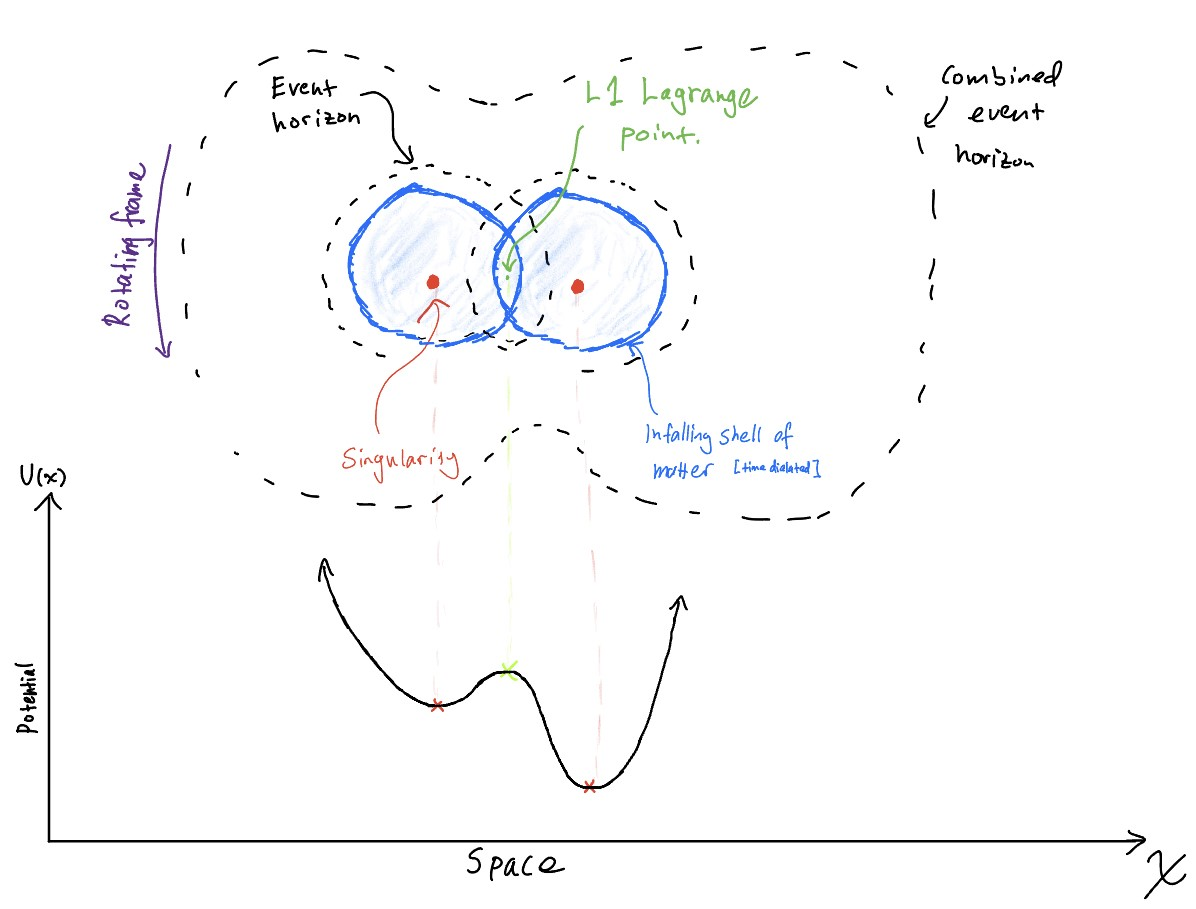
\includegraphics[width=\textwidth]{preliminaries/preliminaries_images/L1_PE.jpeg}

The Lagrange points in a binary system refer to the five specific points in the orbital plane of the two-body system where a small object can maintain a stable or unstable position relative to the two larger bodies. The two bodies could be, for instance, the Earth and the Moon, or the Earth and the Sun. These points are named after the mathematician Joseph-Louis Lagrange.

L1: This point lies between the two larger bodies. It allows an object to essentially 'hover' in that spot relative to the two larger bodies. This is because the gravitational forces from the two larger bodies and the centrifugal force all balance out.

L2: This point lies beyond the smaller of the two bodies, on the line defined by the two larger bodies. Like L1, objects at L2 can stay there due to the balance of the gravitational forces of the two larger bodies and the centrifugal force.

L3: This point lies beyond the larger of the two bodies, on the line defined by the two larger bodies. It is on the opposite side of the larger body from the smaller one.

L4 and L5: These points lie at the third corners of an equilateral triangle whose other corners are defined by the two larger bodies. L4 is ahead of the smaller body in its orbit, and L5 is behind.

Now, regarding stability: L1, L2, and L3 are unstable in the sense that a small perturbation will move the object away from the Lagrange point, and the object will not return. However, they are stable in a different sense: an object close to these points will stay close (though not in a fixed position) if it has a small "velocity" relative to the point. This is known as metastability.

L4 and L5, on the other hand, are stable under small perturbations, provided the mass ratio of the two main bodies is greater than approximately 24.96. This condition is met for many significant cases, such as the Earth-Moon system and the Sun-Jupiter system. If an object is slightly perturbed from L4 or L5, it will move around the Lagrange point but not away from it.

The L1 point, as you mention, is metastable. This means that while an object at L1 might move away if perturbed, an object close to L1 will stay close if it is moving at a small relative speed. This is the principle behind the solar observatories SOHO and ACE, for example, which are in orbits designed to keep them close to the Sun-Earth L1 point.

Astrophysically, this property of metastability has interesting implications for angular momentum accretion. In the vicinity of the L1 point, matter can transition from one body to another due to gravitational forces. This is particularly important in binary star systems, where one star can accrete matter from its companion star if the companion overflows its Roche lobe - the region of space around a star where material is gravitationally bound to that star. The point at which this overflow occurs is often near the L1 point.

The matter that flows through the L1 point carries with it angular momentum. As this matter accretes onto the recipient star, it can form an accretion disk around the star, and the process of accretion can lead to a redistribution of angular momentum within the system. This can have various effects, such as changing the spin rates of the stars and altering the orbital parameters of the binary system. In extreme cases, this angular momentum transfer can lead to phenomena such as mass transfer instabilities, nova outbursts, or even type Ia supernovae.